

\documentclass[sigconf,nonacm]{acmart}

\settopmatter{printacmref=false, printccs=false, printfolios=false}
\renewcommand\footnotetextcopyrightpermission[1]{}
\pagestyle{empty} % Suppress headers and footers globally

\usepackage{fancyhdr}
\fancypagestyle{empty}{
    \fancyhf{} % Clear header/footer
    \renewcommand{\headrulewidth}{0pt}
    \renewcommand{\footrulewidth}{0pt}
}
\usepackage{amsmath, amssymb}

% Packages
\usepackage{amsmath, amssymb, amsfonts}
\usepackage{graphicx}
\usepackage{balance}
\usepackage{caption}
\usepackage{algorithm}
\usepackage{algpseudocode}
\usepackage{bm} % For bold math symbols
\usepackage{multicol} % For multi-column layouts (if needed)
\usepackage{mathtools} % Additional math features

% Begin Document
\begin{document}

\title{Geometric Data Analysis: Fake News Detection on Social Media using Geometric Deep Learning\\
\vspace{0.5em}} % Adjust spacing if needed after removing subtitle


\author{Niloo Sahebalzamany}
\affiliation{
  \institution{Columbia University}
  \country{}
}
\email{ns2434@caa.columbia.edu}

\author{Clément Rouvroy}
\affiliation{
  \institution{Ecole normale supérieure}
  \country{ }
}
\email{clement.rouvroy@ens.psl.eu}

\author{Grégoire Le Corre}
\affiliation{
  \institution{Ecole normale supérieure}
  \country{}
}
\email{gregoire.le.corre@ens.psl.eu}



% Updated abstract
\begin{abstract}
This report looks at the application of GNN to detect fake news based on \cite{monti2019fakenewsdetectionsocial}. Social media platforms have revolutionized news consumption but have simultaneously amplified the spread of fake news, posing critical challenges to information integrity. Traditional detection methods relying on content analysis struggle with nuanced misinformation requiring contextual or common-sense understanding. This paper introduces a novel geometric deep learning framework leveraging graph-based propagation features for fake news detection. By analyzing propagation dynamics, user behaviors, and network structures, our model achieves language independence and resistance to adversarial attacks. Tested on verified Twitter datasets spanning 2013–2018, our method attains 92.7\% ROC AUC in URL-wise classification and demonstrates reliable early detection within hours of news dissemination. This study highlights the potential of propagation-based detection as a robust alternative or complement to content-focused approaches, with applications extending to scalable, real-time solutions for combating misinformation on social media.
\end{abstract}

\maketitle

\section{Introduction}
Social media platforms are prominent sources of news today, offering rapid dissemination but posing significant risks such as the spread of fake news. Fake news often relies on misinformation and manipulation, challenging traditional content-based detection methods. Geometric deep learning provides a promising alternative, analyzing how news spreads within social networks rather than its content. This method leverages graph-based data structures to integrate content, user profiles, and propagation patterns, allowing early and accurate fake news detection. This report explores these methods and their effectiveness using real-world datasets.

\section{Literature Review}
\subsection{Previous Approaches to Fake News Detection}
Content-based methods focus on linguistic features to identify deceptive cues, while social context-based approaches consider user demographics and interactions. Propagation-based methods leverage the spread patterns of news across social networks, offering greater resilience to adversarial attacks.

\subsection{Geometric Deep Learning in Social Media Analysis}
Geometric deep learning has been applied to tasks like social network analysis, misinformation detection, and community detection. By generalizing neural networks to non-Euclidean data, these methods efficiently model graph-structured information.

\section{Methodology}

Fake news detection is formulated as a graph classification problem, where nodes represent users and edges capture social interactions or news propagation paths.

\subsection{Data}

The dataset consists of annotated fake and real news stories spread on Twitter between 2013 and 2018, verified by professional fact-checking organizations such as Snopes, PolitiFact, and Buzzfeed. Each story is linked to a URL and propagated as a cascade, defined by a source tweet referencing the URL and its subsequent retweets. The dataset includes the following:

\begin{itemize} \item \textbf{Claims}: 1,084 labeled claims, each linked to an article and classified as true or false. \item \textbf{Cascades}: 158,951 cascades representing propagation patterns of news on Twitter. \item \textbf{Users and Connections}: 202,375 unique users connected by 2,443,996 edges in the Twitter social graph. \end{itemize}

\textbf{Features.} The dataset provides rich feature sets categorized as: \begin{itemize} \item \textbf{User profile:} Includes geolocalization, language, profile settings, verification status, word embeddings of self-descriptions, and account creation dates. \item \textbf{User activity:} Metrics such as the number of favorites, lists, and statuses. \item \textbf{Network and spreading:} Social connections (followers and friends), cascade tree structures, retweet timestamps, source devices, and counts of replies, quotes, favorites, and retweets for the source tweet. \item \textbf{Content:} Word embeddings of tweet content and hashtags. \end{itemize}

\textbf{Cascade Size.} The average cascade size is 2.79 tweets, with a significant portion of cascades being small. To focus on meaningful propagation patterns, cascades with fewer than six tweets were excluded from some experiments.

\textbf{Credibility and Polarization.} Users were assigned a credibility score ranging from -1 to +1, reflecting the proportion of true versus fake news they propagated. The social network demonstrated significant polarization, with credible (blue) and non-credible (red) users forming distinct communities.
\subsection{Model Architecture}

The proposed model is a Graph Convolutional Network (GCN) designed for fake news classification using propagation patterns. It integrates heterogeneous data, including user profiles, tweet content, and social interactions, into a unified framework. The architecture consists of the following components:

\textbf{Input Graph Representation:}  
Each news cascade is represented as a directed graph. The nodes represent tweets or users, and are characterized by several features:
- \textit{User Activity:} Features such as retweet count, account age, and the number of friends and followers.
- \textit{Content Embeddings:} 200-dimensional GloVe embeddings pre-trained on Twitter data.
- \textit{Metadata:} Includes timestamps, verified status, and geolocation.

The edges in the graph capture propagation relationships such as retweets or follows, with each edge enriched with features indicating the type and direction of interaction.

\textbf{Graph Convolutional Layers:}  
The model employs two graph convolutional layers to compute node embeddings:
- Each layer outputs 64-dimensional feature vectors for the nodes.
- A single-head attention mechanism is applied to assign weights to edges based on their significance.
- Scaled Exponential Linear Unit (SELU) activation is applied after each convolution operation.

\textbf{Pooling Layer:}  
Mean pooling aggregates the node-level embeddings into a single graph-level feature vector that summarizes the cascade.

\textbf{Fully Connected Layers:}  
The graph-level representation is passed through the following layers:
- A dense layer reduces the feature dimension to 32.
- A final output layer with 2 units performs binary classification (fake/true news).
\begin{table*}[t]
    \centering
    \caption{Dataset Statistics}
    \begin{tabular}{lcccc}
        \toprule
        \textbf{Dataset} & \textbf{\#Graphs (\#Fake)} & \textbf{\#Total Nodes} & \textbf{\#Total Edges} & \textbf{\#Avg. Nodes per Graph} \\
        \midrule
        Politifact (POL) & 314 (157) & 41,054 & 40,740 & 131 \\
        Gossipcop (GOS)  & 5464 (2732) & 314,262 & 308,798 & 58 \\
        \bottomrule
    \end{tabular}
    \label{tab:data_statistics}
\end{table*}
\textbf{Loss and Optimization:}  
- The model is trained using hinge loss, as it outperformed cross-entropy in early experiments.
- AMSGrad is used as the optimizer, with a learning rate of \( 5 \times 10^{-4} \).
- Dropout regularization is applied to fully connected layers to prevent overfitting.
- Training is performed for 25,000 iterations for URL-wise classification and 50,000 iterations for cascade-wise classification, with a mini-batch size of 1.

\textbf{Early Propagation Settings:}  
The model can classify news based on early propagation patterns by considering truncated cascades:
- Cascades are truncated at intervals (e.g., 2 hours, 7 hours, and 24 hours) to analyze detection performance over time.
- A minimum cascade size of 6 tweets is required for classification, as smaller cascades lack sufficient propagation patterns.

This architecture leverages propagation dynamics, graph structure, and multi-modal features to provide robust and early detection of fake news.




\subsection{Mathematical Framework of Geometric Deep Learning}
Geometric deep learning generalizes classical deep learning techniques to non-Euclidean domains such as graphs and manifolds. This paper leverages these techniques to model social media propagation patterns as graph-structured data, enabling the detection of fake news.

\paragraph{Graph Representation}
A social media cascade is represented as a graph \( G = (V, E) \), where \( V \) denotes the nodes (tweets or users), and \( E \) denotes the edges (retweets, follows, or interactions). The adjacency matrix \( \bm{A} \) encodes these connections, while the degree matrix \( \bm{D} \) represents node degrees. The normalized graph Laplacian \( \bm{L}_{\text{norm}} \) is:
\[
\bm{L}_{\text{norm}} = \bm{I} - \bm{D}^{-1/2} \bm{A} \bm{D}^{-1/2}.
\]

\paragraph{Graph Convolution}
The model utilizes spatial graph convolutions, which iteratively aggregate features from neighboring nodes. For a node \( i \), the feature update at layer \( l+1 \) is:
\[
\bm{h}_i^{(l+1)} = \sigma \left( \sum_{j \in \mathcal{N}(i)} \frac{1}{c_{ij}} \bm{W}^{(l)} \bm{h}_j^{(l)} \right),
\]
where \( \bm{h}_j^{(l)} \) is the feature vector of node \( j \) at layer \( l \), \( \bm{W}^{(l)} \) is the learnable weight matrix, \( c_{ij} \) is a normalization constant, and \( \sigma \) is the activation function (e.g., Scaled Exponential Linear Unit, SELU).

\paragraph{Attention Mechanism}
Graph Attention Networks (GATs) enhance traditional convolution by dynamically weighting edges. The attention coefficient \( \alpha_{ij} \) for nodes \( i \) and \( j \) is computed as:
\[
\alpha_{ij} = \frac{\exp(\text{LeakyReLU}(\bm{a}^\top [\bm{W} \bm{h}_i || \bm{W} \bm{h}_j]))}{\sum_{k \in \mathcal{N}(i)} \exp(\text{LeakyReLU}(\bm{a}^\top [\bm{W} \bm{h}_i || \bm{W} \bm{h}_k]))},
\]
where \( \bm{a} \) is a learnable vector, and \( [\cdot || \cdot] \) denotes concatenation.

\paragraph{Propagation Modeling}
News propagation paths are constructed by combining retweet timestamps and social graph structures. These paths define the graph \( G \), where node and edge features encode user activity, content, and propagation dynamics. This graph is processed iteratively by the geometric deep learning model to learn propagation-specific patterns indicative of fake or real news.


\subsection{Model Settings}

The model operates in two distinct settings:
\begin{itemize}
    \item \textbf{URL-wise Classification}: In this setting, the model aggregates information from all cascades linked to a specific URL to determine its veracity. On average, each URL has 141 cascades.
    \item \textbf{Cascade-wise Classification}: Here, the model evaluates a single cascade independently to predict the label of its associated URL. Cascades with fewer than six tweets are excluded to ensure sufficient propagation data.
\end{itemize}

Each setting is trained using supervised learning, with hinge loss as the objective function. The URL-wise setting benefits from aggregated data, while the cascade-wise approach focuses on individual propagation patterns, making it more challenging but also more granular.

\textbf{Summary of Results.}
The model demonstrated strong performance across both settings, as measured by the area under the ROC curve (ROC AUC):
\begin{itemize}
    \item \textbf{URL-wise Classification}: Achieved an average ROC AUC of $92.70\%$, indicating high accuracy when aggregating information from all cascades linked to a URL.
    \item \textbf{Cascade-wise Classification}: Despite the increased difficulty of evaluating single cascades, the model achieved an impressive average ROC AUC of $88.30\%$.
\end{itemize}

Further analysis revealed that cascade size significantly impacts classification performance. Larger cascades provide more reliable propagation patterns, with a minimum threshold of six tweets per cascade optimizing results. Moreover, the model exhibited robust early detection capabilities, achieving above $90\%$ accuracy within a few hours of news propagation in the URL-wise setting.

\section{Implementation}

Our implementation is publicly accessible here \cite{github}. We employed the model architecture described in \cite{monti2019fakenewsdetectionsocial} as detailed in Section 3.2, with a modification to the batch size, which we set to 128 instead of 1 to improve training efficiency and handle larger data batches.

In this study, we leverage URL-wise classification to determine the veracity of a news story by aggregating information from all Twitter cascades associated with a given URL. This approach aligns naturally with the organic structure of our dataset, which is inherently organized at the URL level. When utilizing all available features, the model achieved a robust Area Under the Receiver Operating Characteristic curve (AUC-ROC) score of 96\%, underscoring the efficacy of feature integration in enhancing classification performance.

\textbf{Data:} The dataset used by Marti et al. is not publicly available. Instead, we leveraged the publicly accessible dataset introduced by \cite{10.1145/3404835.3462990}, which differs slightly in its construction. Specifically, each news diffusion on Twitter is modeled as an undirected graph, with the news itself serving as the root node (rather than the tweet citing it). Nodes directly connected to the root represent tweets that reference the news URL, while the edges between these nodes capture the retweet relationships of those initial tweets.

\textbf{Node Features:} In addition to the graph structure, we incorporated various node features derived from the User Preference-aware Fake News Detection dataset (UPFD). These features include:
\begin{itemize}
    \item \textbf{Spacy:} A 300-dimensional word2vec embedding representing the historical content of the user's profile.
    \item \textbf{BERT:} A 768-dimensional embedding capturing the semantic content of the user’s profile using BERT.
    \item \textbf{Profile:} A 10-dimensional vector encapsulating key profile attributes, including the username, Twitter handle, and follower count.
    \item \textbf{Content:} A concatenated vector combining:
    \begin{enumerate}
        \item A 300-dimensional word2vec embedding of the tweet's content.
        \item The 10-dimensional profile vector described above.
    \end{enumerate}
\end{itemize}

\begin{figure}
    \centering
    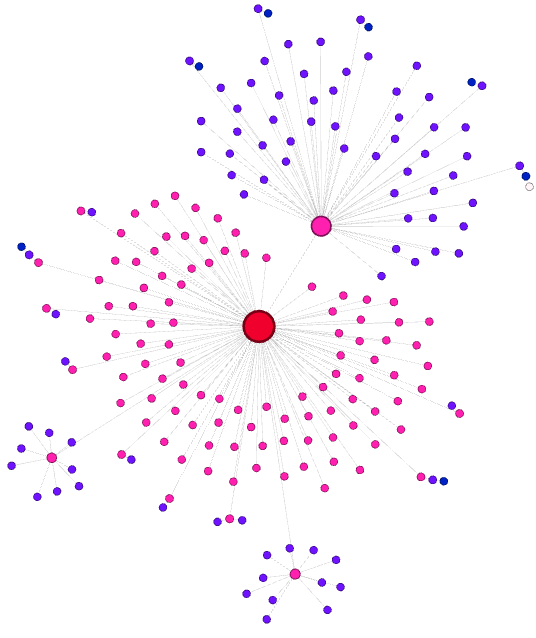
\includegraphics[scale=0.3]{graph_528_label_0_better_representation.png}
    \caption{Graph representing an URL cascade. Color depends on depth (i.e. number of reweet) and size represents degree. The big node red is the URL, node it pink tweets containing URL, node in blue first retweet, ...}
    \label{fig:url_cascade}
\end{figure}

\begin{figure}
    \centering
    \includegraphics[scale=0.3]{Diagramme_bâton_cascades.png}
    \caption{Breakdown of the number of cascading URLs by size (number of nodes)}
    \label{fig:graph_repartition}
\end{figure}

Figure \ref{fig:url_cascade} provides a visualization of an example URL cascade from our dataset, highlighting its graph representation. Table~\ref{tab:data_statistics} and Figure \ref{fig:graph_repartition} summarizes the dataset statistics, offering a detailed overview of its composition and key characteristics.



\section{Experiments}


This study follows the methodology of \cite{monti2019fakenewsdetectionsocial} to explore the impact of different feature combinations on the performance of our model using the UPFD dataset. We performed an ablation study to evaluate how various feature sets contribute to model performance. The results, shown in Figure~\ref{fig:ablation_results}, reveal significant improvements as specific features are incorporated into the model.

The inclusion of user profile and preferences resulted in an ROC-AUC score of 0.88, demonstrating the importance of user-specific contextual information. Further isolating the profile features led to a substantial increase in performance to 0.93, underscoring their predictive strength. When all features—profile, preferences, content, and interactions—were combined, the model achieved a score of 0.96, showcasing the positive impact of a diverse feature set.

However, contrary to expectations, the best performance of 0.98 was observed when only the profile and content features were used together. This result suggests that while adding additional features provides some improvements, the combination of profile and content features outperforms the full set of four features. The inclusion of all four features introduced some redundancy, which may have detracted from the model’s overall performance. 

These findings align with the observations made by \cite{monti2019fakenewsdetectionsocial}, where feature selection played a pivotal role in enhancing model accuracy. In our case, the profile and content features, when combined, provided the most effective representation of both user-specific and tweet-specific contexts, thereby achieving the highest predictive accuracy. This highlights the importance of optimizing feature combinations and avoiding unnecessary complexity, which can lead to diminishing returns. 

Overall, this study emphasizes the critical role of strategic feature engineering. By carefully selecting the most informative features—particularly profile and content—we were able to achieve optimal performance without the added complexity of redundant features.

\section{Extensions}

\subsection{Random Features and the Role of Graph Propagation in Fake News Diffusion}

Building on the idea of propagation and the patterns of tweet diffusion, we explored the effect of using random features in our analysis. This approach aimed to isolate the structural properties of the graph from the influence of carefully crafted features. Notably, despite the randomness of the features, the AUC-ROC score achieved was 0.67, suggesting that the graph itself inherently encodes valuable information.

This finding underscores the critical role of graph structure in distinguishing fake news from legitimate content. The propagation patterns unique to fake news dissemination appear to manifest in the graph topology, independent of specific node-level attributes. For instance, fake news tends to propagate through distinct clusters or patterns of re-sharing that differ significantly from genuine news diffusion. Such differences are captured by the graph's structural properties, reinforcing the idea that graph-based representations can be highly effective for tasks like fake news detection.

The implications of these results are twofold:
\begin{itemize}
    \item \textbf{Feature Agnosticism:} Even without domain-specific features, the graph's structural information contributes meaningfully to classification performance. This suggests that algorithms leveraging the graph alone, such as Graph Neural Networks (GNNs) or propagation-based heuristics, could yield robust results in detecting fake news.
    \item \textbf{Future Directions:} Future work could focus on integrating random features with learnable embeddings to further disentangle the contributions of structure and content. Moreover, analyzing specific subgraph patterns or motifs prevalent in fake news diffusion might help refine detection strategies further.
\end{itemize}

\subsection{Impact of Regularization (Weight Decay) on Model Performance}

Incorporating regularization techniques, particularly weight decay, was another avenue we explored to improve the robustness and generalization of our models. Weight decay, by penalizing large weights, aims to prevent overfitting and encourage smoother decision boundaries. However, our findings revealed that regularization did not consistently improve the AUC-ROC performance across the majority of models. In some cases, it even led to a decrease in AUC-ROC scores.

This counterintuitive outcome suggests that weight decay may lead to over-regularization in the context of our models. By overly constraining the parameter space, weight decay might prevent the model from capturing subtle patterns in the data that are crucial for distinguishing between fake and genuine news. These results align with the hypothesis that excessive regularization can hinder a model's ability to effectively learn from the data, especially when the underlying patterns are complex and nuanced, as is often the case with fake news detection.

The key takeaways from this observation are as follows:
\begin{itemize}
    \item \textbf{Trade-off Between Generalization and Expressiveness:} Regularization introduces a bias toward simpler models, which can be beneficial for noisy data. However, in our case, the reduction in expressiveness outweighed the benefits, leading to suboptimal performance.
    \item \textbf{Sensitivity to Model Complexity and Data Characteristics:} The adverse impact of weight decay highlights the importance of tailoring regularization techniques to the specific characteristics of the data and the model. The diffusion patterns in fake news graphs, combined with potentially high-dimensional feature spaces, may require a more nuanced approach to regularization.
    \item \textbf{Future Work on Adaptive Regularization:} Instead of a uniform weight decay penalty, adaptive regularization strategies, such as dropout or layer-specific penalties, could be explored to better balance generalization and expressiveness. Additionally, analyzing the relationship between regularization strength and graph-based feature importance may shed further light on the interplay between model constraints and structural learning.
\end{itemize}

\vspace{1em} % Adds spacing for emphasis

In summary, our extensions provide valuable insights into the interplay between graph structure, feature engineering, and regularization in fake news detection. The strong performance of random features highlights the intrinsic value of graph-based propagation patterns, while the mixed results with weight decay emphasize the need for a careful calibration of regularization strategies. These findings open avenues for further exploration into the synergy between graph representation learning and model optimization techniques in combating misinformation.



\section{Limitations}

This study presents several limitations that warrant consideration, particularly regarding the generalizability and contextual applicability of the proposed model:

\begin{itemize}
    \item \textbf{Dataset Specificity}: The model was trained using a Twitter dataset annotated with fact-checking labels. Consequently, its ability to generalize to other social media platforms, particularly those with less structured or differently moderated environments, remains uncertain.

    \item \textbf{Dependence on Propagation Patterns}: The model heavily relies on propagation dynamics, which may not be as prominent or accessible in less networked or sparsely connected settings. This reliance could limit its utility in platforms where such patterns are difficult to observe or quantify.

    \item \textbf{Temporal Degradation}: Findings indicate that the model's performance degrades over time, highlighting the necessity of frequent retraining to sustain accuracy, especially in the context of rapidly evolving news ecosystems and information landscapes.

    \item \textbf{Dataset Comparability}: Unlike \cite{monti2019fakenewsdetectionsocial}, who utilized a fact-checker-verified Twitter dataset, this study employs a dataset introduced by \cite{10.1145/3404835.3462990}, which represents news diffusion using undirected graphs with news URLs as root nodes. This methodological variation might constrain the direct comparability of results across different datasets, complicating broader benchmarking efforts.

    \item \textbf{Dependence on Graph Richness and Data Quality}: The effectiveness of the model is contingent on the availability of detailed graph structures and high-quality user profile features. This dependency could limit the model’s generalizability to other datasets or platforms characterized by sparse, noisy, or incomplete data.
\end{itemize}

These limitations underscore the need for further exploration into adaptive methodologies and cross-platform evaluations to enhance the robustness and applicability of the model.



\section{Results and Discussion}

The effectiveness of the proposed model was evaluated using a dataset that introduced novel characteristics and advanced feature engineering. This section discusses the model's performance, the significance of individual feature sets, and insights gained through analytical experiments.

\subsection{Model Performance}

The model demonstrated strong predictive capabilities, achieving a 96\% AUC-ROC for URL-wise classification when leveraging the full suite of features. This result underscores the robustness of integrating user profiles, content attributes, and propagation patterns. Notably, these findings align with prior studies emphasizing the efficacy of such multifaceted approaches.

Interestingly, the dataset analysis revealed nuanced interactions among the feature sets. While propagation patterns and user profiles were corroborated as critical components consistent with \cite{monti2019fakenewsdetectionsocial}'s observations, the combination of profile and content features alone yielded the highest AUC-ROC at 98\%. This suggests potential redundancies in the simultaneous integration of all feature sets. These insights indicate that strategic feature selection may enhance computational efficiency without compromising accuracy.

\subsection{Feature Analysis}

A detailed ablation study further validated the importance of specific feature groups. Profile features, such as BERT embeddings and follower counts, emerged as pivotal for distinguishing fake news. These results resonate with prior research, reaffirming the value of user-centric metrics in addressing misinformation.

To probe the underlying discriminative power of graph-based representations, experiments using random features were conducted. Remarkably, even with the absence of domain-specific information, the graph structure achieved a 67\% AUC-ROC. This finding highlights the intrinsic ability of graph topology to capture propagation dynamics, reinforcing the hypothesis that structural characteristics alone offer significant discriminatory potential between fake and authentic news dissemination patterns.

\subsection{Implications and Future Directions}

The findings underscore the importance of leveraging graph-based insights and user profile attributes in detecting misinformation. However, the observed redundancies in feature integration suggest the need for further exploration into feature optimization strategies. Future work could focus on developing adaptive feature selection mechanisms to refine model efficiency while maintaining or enhancing predictive performance.


\section{Conclusion and Future Work}

This study demonstrates the potential of geometric deep learning in fake news detection, effectively integrating user profiles, activity patterns, propagation dynamics, and semantic content. The model achieves high predictive accuracy and adaptability across diverse datasets, showcasing its robustness and early detection capabilities.

\subsection*{Achievements}
The proposed approach successfully generalized beyond Twitter data, maintaining strong performance while revealing the nuanced contributions of graph-based propagation and user-level features.

\subsection*{Challenges}
Key challenges included:
\begin{itemize}
    \item Data scarcity and structural differences across networks.
    \item Biased propagation patterns, which impacted model consistency.
\end{itemize}

\subsection*{Future Work}
To address these challenges and extend the study, future directions include:
\begin{itemize}
    \item \textbf{Cross-Platform Validation}: Extend the model to multilingual and platform-agnostic datasets (e.g., Facebook, Instagram) to evaluate generalizability.
    \item \textbf{Temporal Adaptation}: Implement dynamic retraining strategies to counteract model aging and adapt to evolving news ecosystems.
    \item \textbf{Feature Engineering}: Explore advanced embedding techniques and feature selection methods to refine performance and reduce redundancy.
    \item \textbf{Hybrid Approaches}: Investigate methods that combine propagation-based and content-based analyses to enhance accuracy and adversarial resilience.
    \item \textbf{Graph Analysis and Regularization}: Study graph motifs specific to fake news diffusion and apply adaptive regularization techniques to balance generalization and expressiveness.
\end{itemize}

This work establishes a strong foundation for advancing fake news detection through innovative graph-based methodologies, paving the way for more interpretable, resilient, and scalable solutions.

\bibliographystyle{ACM-Reference-Format}
\bibliography{references}

\end{document}
